% ||||||||||||||||||||||||||||||||||||||||||||||
% Capitulo de Resultados Preliminares
% ||||||||||||||||||||||||||||||||||||||||||||||

\chapter{Análine de Resultados}

Nesse capítulo são apresentados os resultados preliminares das técnicas desenvolvidas, mostrando a viabilidade das mesmas. Os resultados 
foram descritos na mesma sequência que foram estudados no capítulo de revisão bibliográfica.

%++++++++++++++++++++++++++++++++++++++++++++++++++++++++++++++++
% 
%++++++++++++++++++++++++++++++++++++++++++++++++++++++++++++++++

\subsection{Análise dos Resultados de Laboratório}

Ao se aplicar a técnica t-SNE nos dados, foi possível se obter 2 mapas 2D a partir de dados de elevada dimensão. O primeiro, que
utilizou como entrada os dados no domínio do tempo, pode ser visto na figura \ref{fig:t-sne-1}.

\begin{figure}[H]
    \caption{Clusters resultantes utilizando a técnica t-SNE no domínio do tempo.}
    \begin{center}
        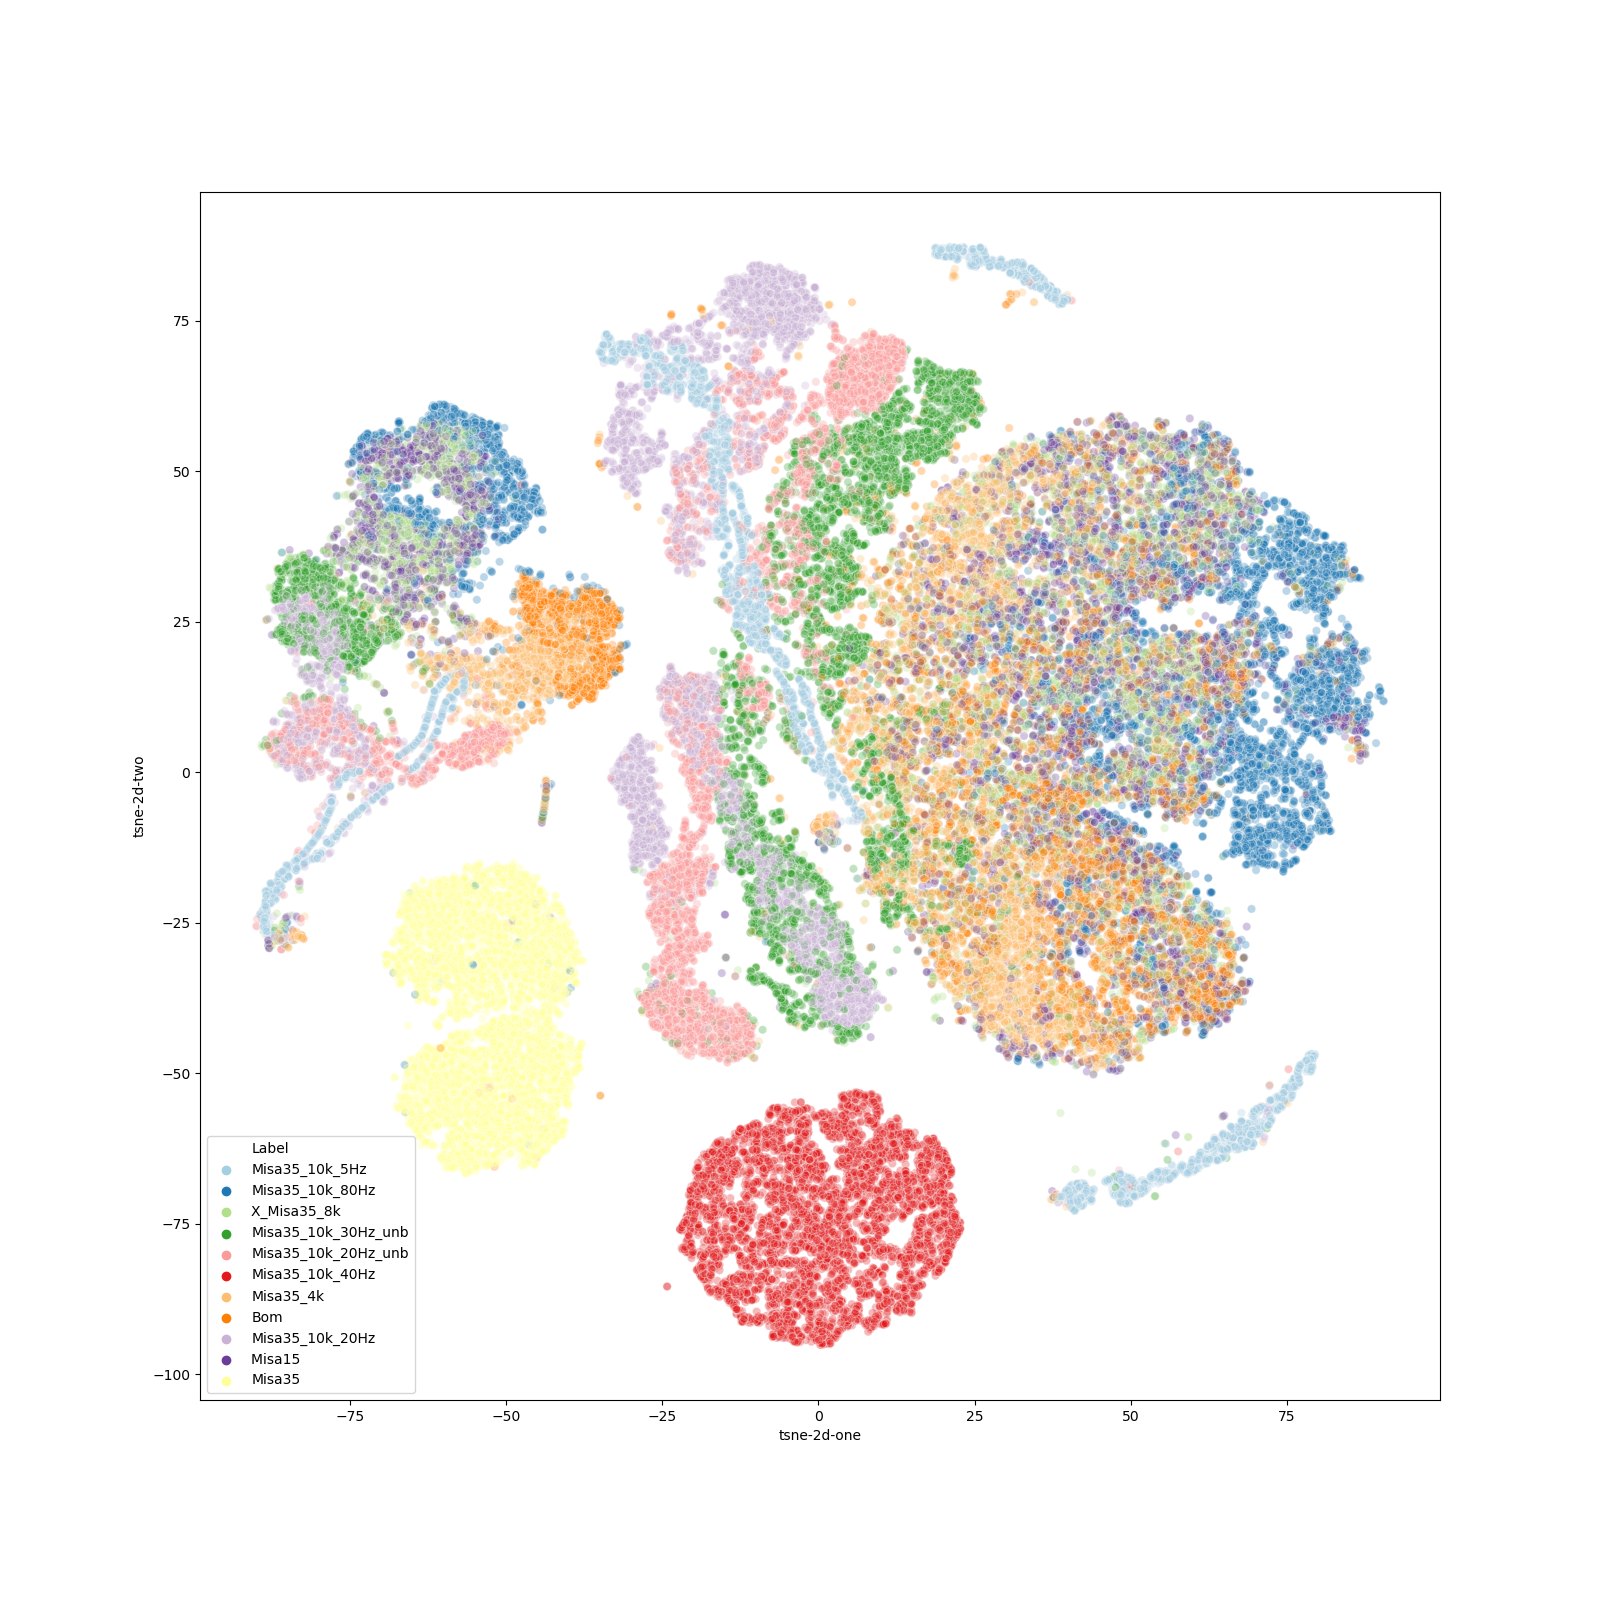
\includegraphics[scale=.25]{resultados/img/t-sne-1.png}
    \end{center}
    \fonte{Elaborado pelo Autor.} 
    \label{fig:t-sne-1}
\end{figure}

Como podemos observar, apenas um cluster teve uma formação mais adequada, do teste chamado "Misa35\_10k\_40Hz". Os demais, ficaram todos
dispersos, não sendo muito conclusivo para isolar todas as falhas. Ao se aplicar a FFT e levar os dados ao domínio do tempo e aplicar o
algoritmo t-SNE também, observa-se a formação do mesmo cluster, não sendo possível ver outro, exatamente como no domínio do tempo. Isso pode
ser visto na figura \ref{fig:fft-t-sne-1}. 

\begin{figure}[H]
    \caption{Clusters resultantes utilizando a técnica t-SNE no domínio da frequência.}
    \begin{center}
        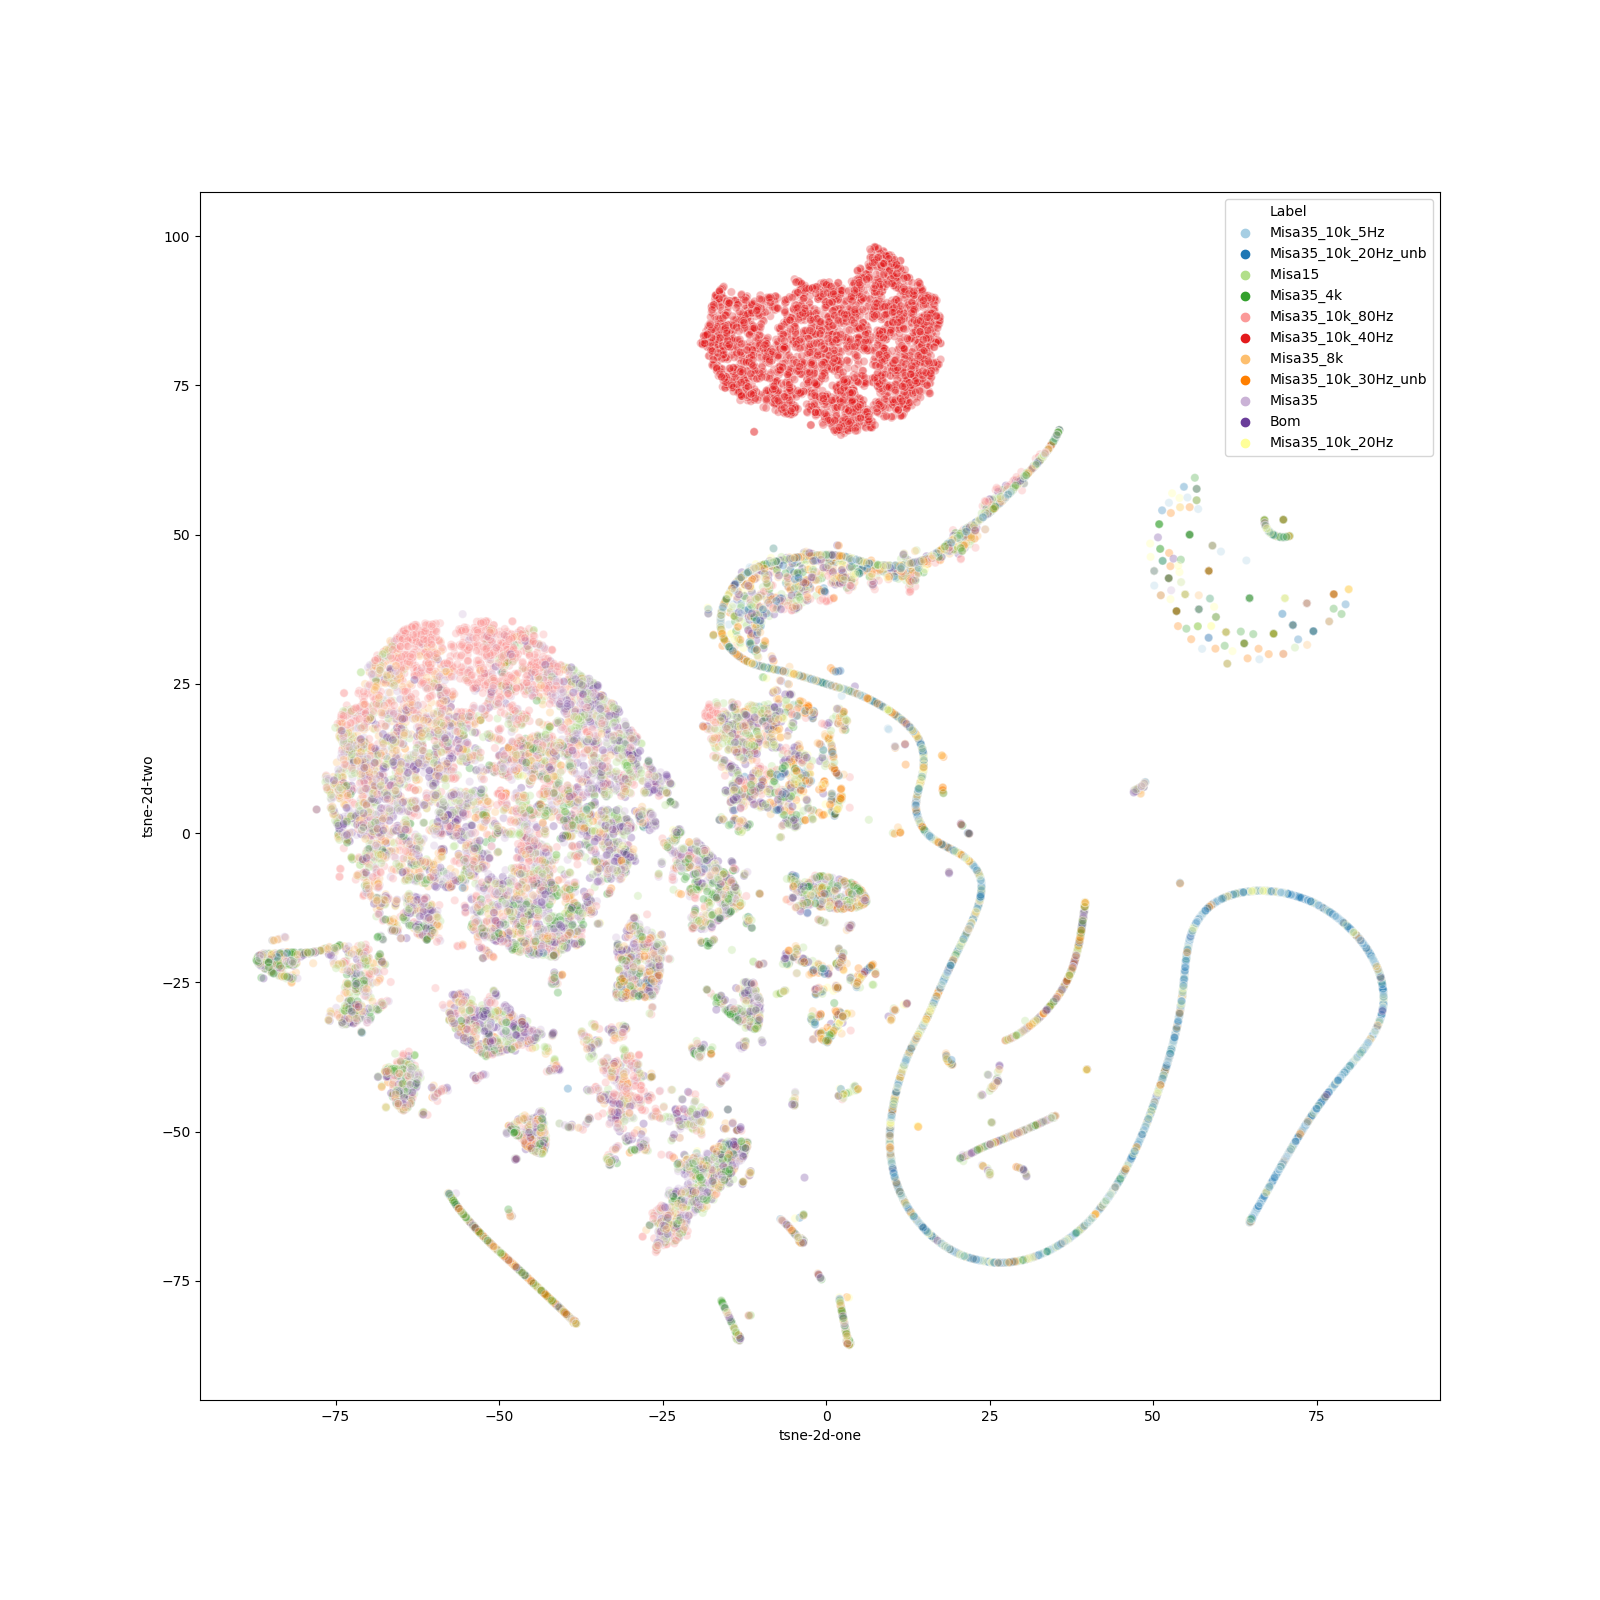
\includegraphics[scale=.25]{resultados/img/fft-t-sne-1.png}
    \end{center}
    \fonte{Elaborado pelo Autor.} 
    \label{fig:fft-t-sne-1}
\end{figure}

Essa técnica não se mostrou muito eficaz em clusterizar a maioria dos dados, mas o comportamento de um deles é semelhante independentemente
do domínio dos dados de entrada.

A outra proposta de aprendizagem de máquina apresentou resultados significativos, onde o K escolhido foi 4 pois, são 4 os tipos de
características, sendo elas: motor bom, desalinhamento de 15 mils, 35 mils e desbalanceamento. A figura \ref{fig:kmeans2} apresenta o mapa
dos resultados.

\begin{figure}[H]
    \caption{Clusters resultantes utilizando a técnica K-means.}
    \begin{center}
        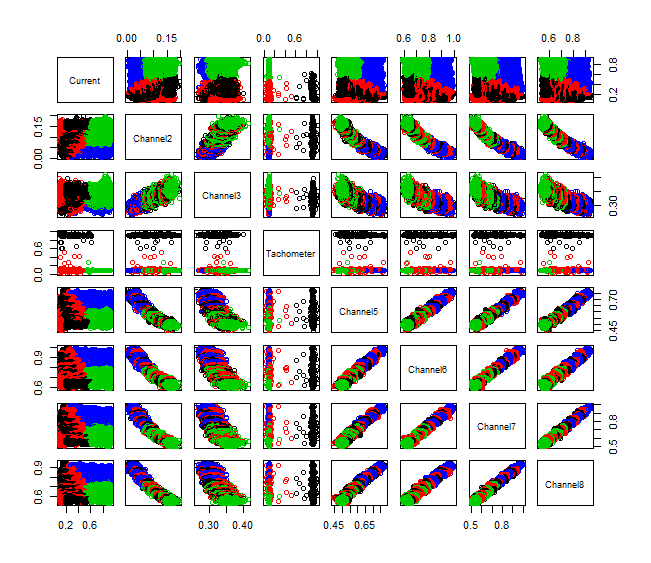
\includegraphics[scale=.65]{resultados/img/kmeans2.png}
    \end{center}
    \fonte{Elaborado pelo Autor.} 
    \label{fig:kmeans2}
\end{figure}

Onde \textit{Current} é a corrente do motor; \textit{Channel2} é o acelerômetro no superior do motor; \textit{Channel3} é o acelerômetro na
frontal do motor; \textit{Tachometer} é o tacômetro; \textit{Channel5} é o acelerômetro na lateral do primeiro mancal; \textit{Channel6} 
é o acelerômetro na frontal do primeiro mancal; \textit{Channel7} é o acelerômetro na lateral do segundo mancal; \textit{Channel8} 
é o acelerômetro na frontal do segundo mancal;


Como podemos ver na coluna e linha da corrente do motor, foram criados 2 clusters perfeitamente isolados na maior parte dos
casos (verde e azul), já o preto e o vermelho em alguns momentos se misturam, mostrando alguma semelhança nos dado das falhas. 
O comportamento um pouco diferente do tacômetro em relação aos outros dados se dá porque ele tem uma frequência proporcional ao do 
inversor de frequência, e por consequência, com a corrente do motor.

E por último, os resultados da técnica ICA, que podem ser vistos na figura \ref{fig:ica}. Como a implementação foi realizada com o uso
de 3 sinais de transdutores distantes uns dos outros, com o objetivo de conseguir separar as fontes dos sinais que estão presentes na
corrente. Na figura é possível ver na primeira parte, os três sinais amostrados, onde o vermelho é a corrente e os outros dois são sinais
de vibração. Já no gráfico do meio, está as fontes separadas via o algoritmo FastICA, com as suas respectivas características. E no último
gráfico, é possível ver a reconstrução dos sinais originais a partir das fontes separadas, apenas com uma mudança de fase no sinal da
corrente, mostrando o perfeito funcionamento da extração das fontes de sinais do sinal de corrente.

\begin{figure}[H]
    \caption{Resultados da separação dos dados utilizando a técnica ICA.}
    \begin{center}
        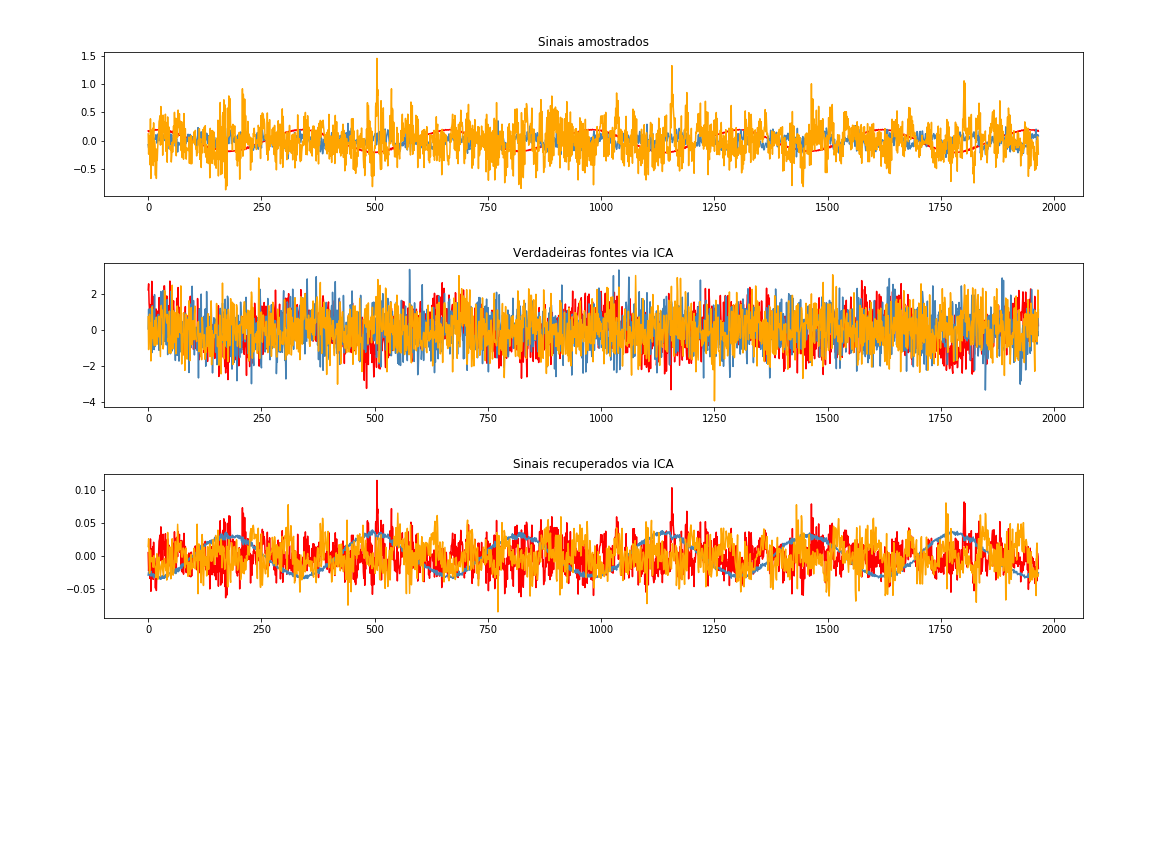
\includegraphics[scale=.4]{resultados/img/ica.png}
    \end{center}
    \fonte{Elaborado pelo Autor.} 
    \label{fig:ica}
\end{figure}


%++++++++++++++++++++++++++++++++++++++++++++++++++++++++++++++++
% 
%++++++++++++++++++++++++++++++++++++++++++++++++++++++++++++++++

\subsection{Análise dos Resultados de Campo}


\begin{figure}[H]
    \caption{Linhas de base e sinais coletados do eixo x.}
    \begin{center}
        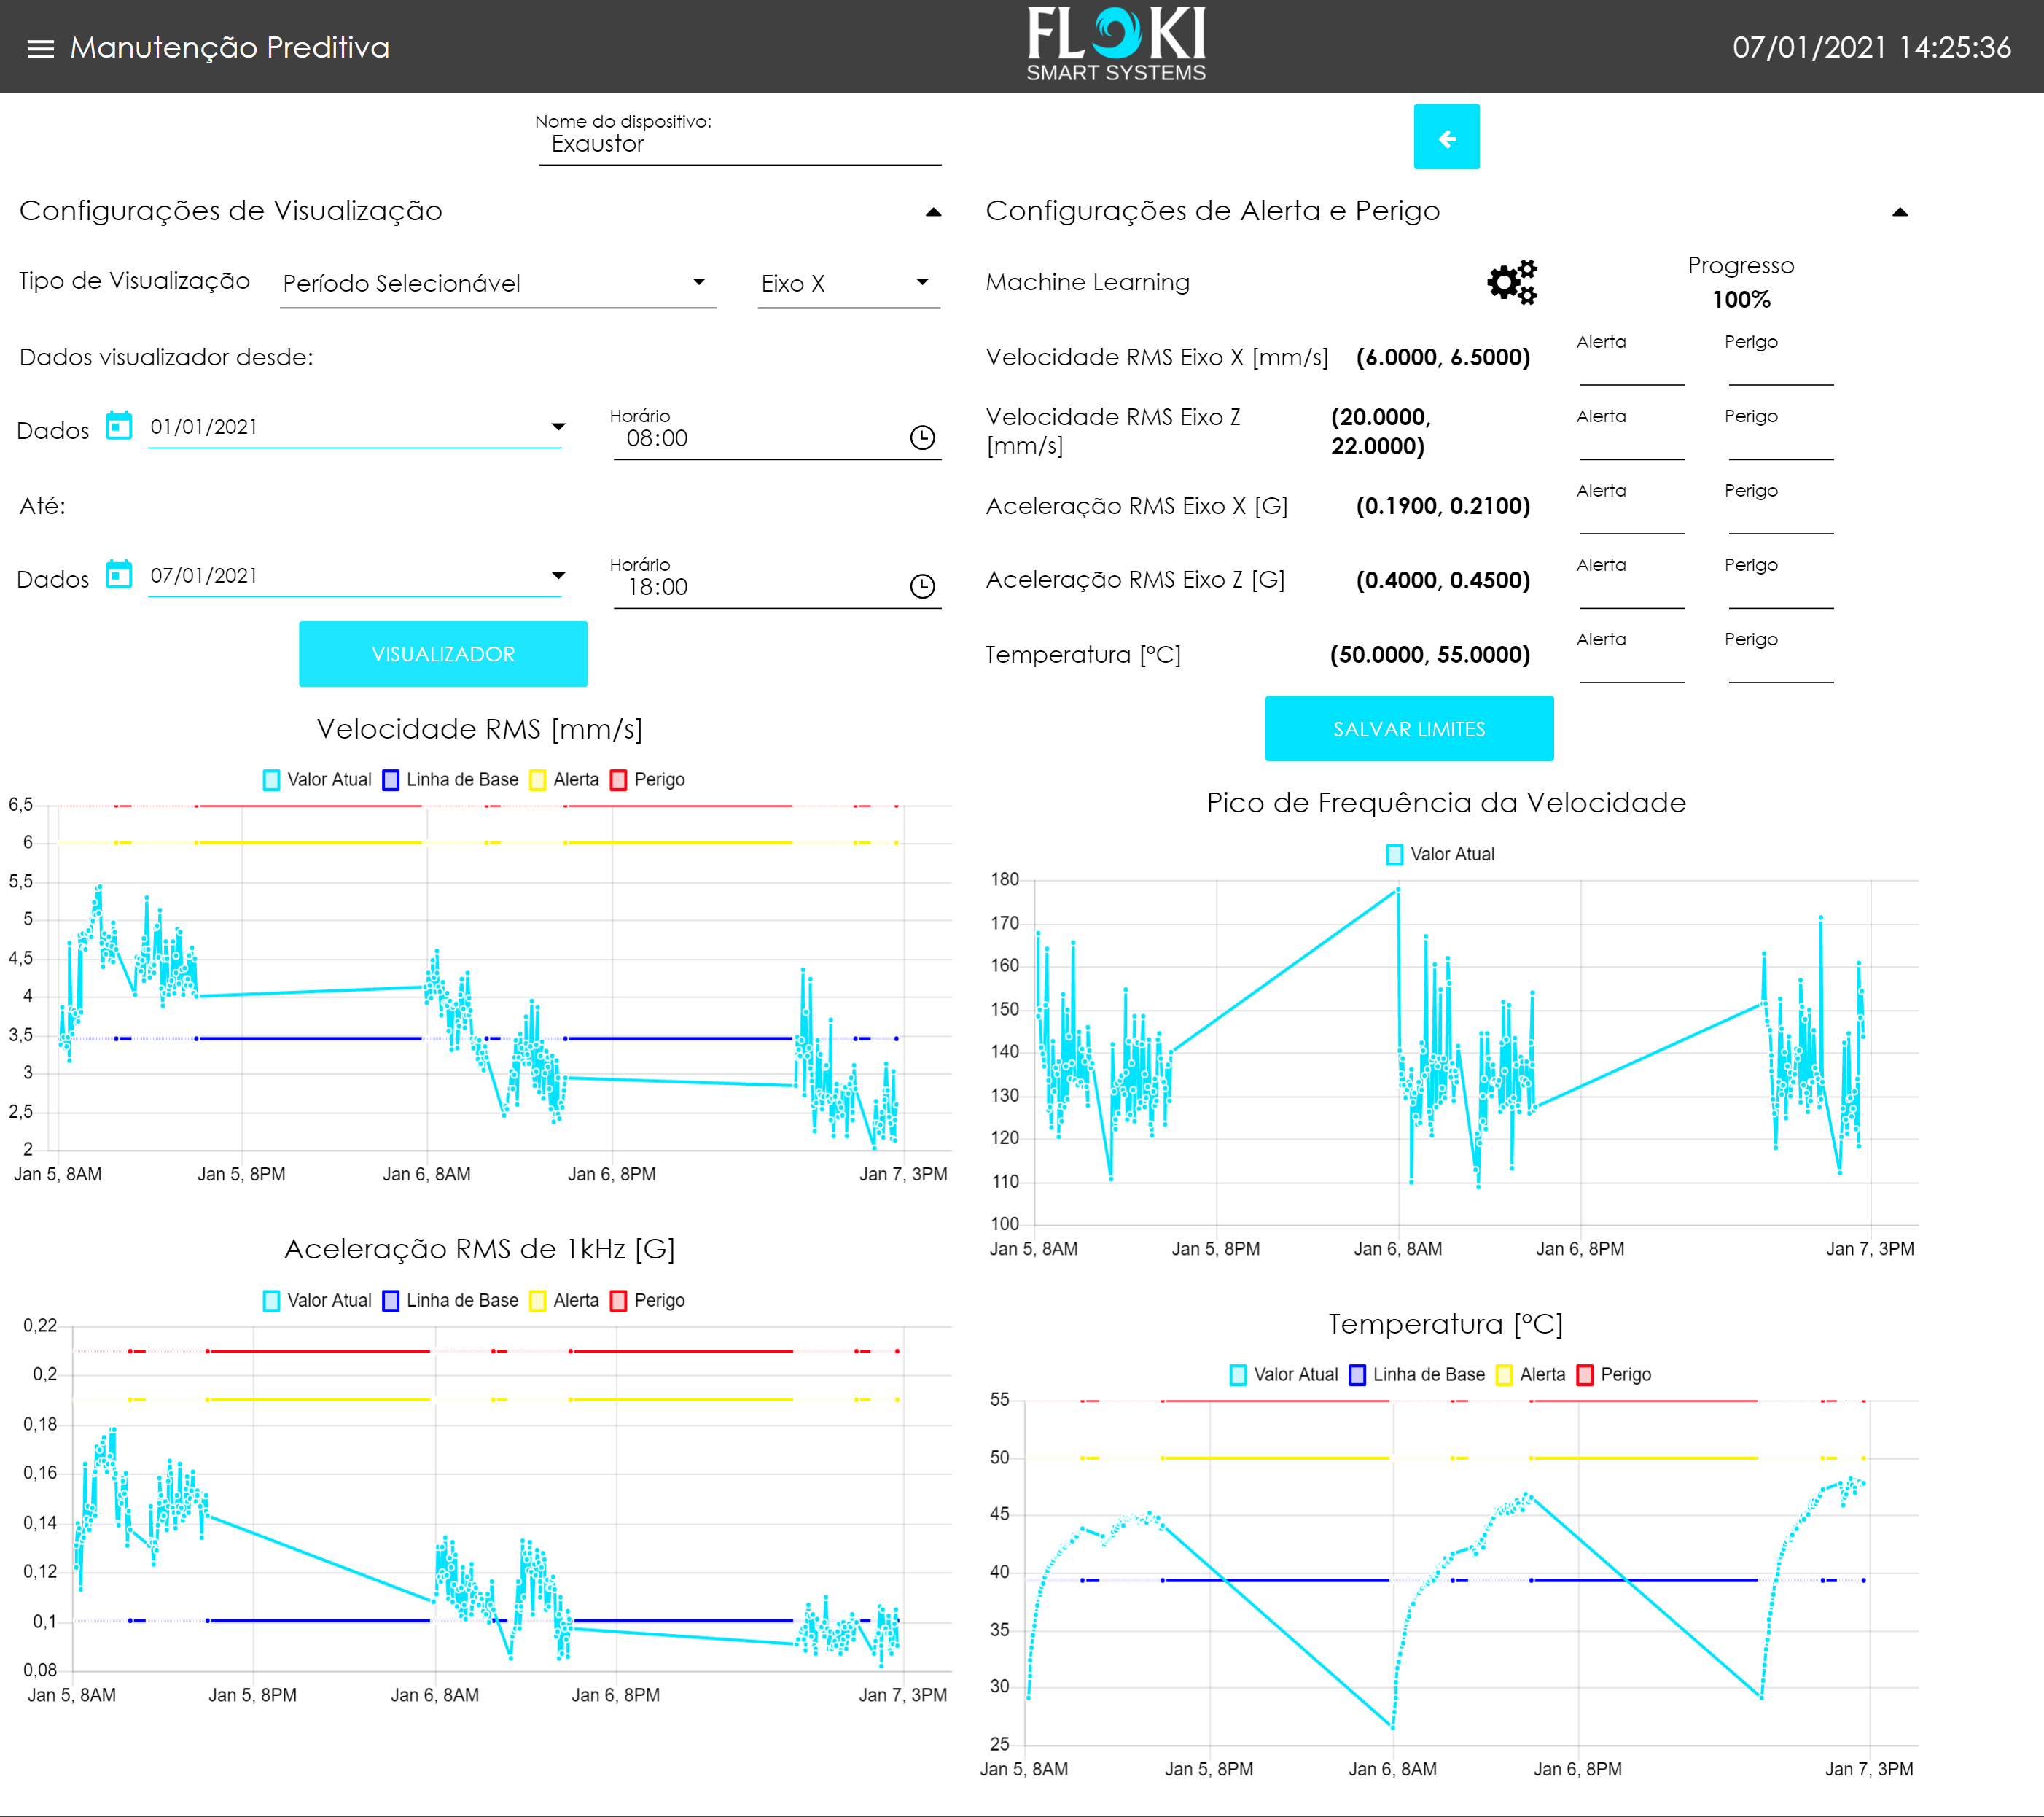
\includegraphics[scale=.15]{resultados/img/drakkar_eixo_x.png}
    \end{center}
    \fonte{Elaborado pelo Autor.} 
    \label{fig:ica}
\end{figure}

\begin{figure}[H]
    \caption{Linhas de base e sinais coletados do eixo z.}
    \begin{center}
        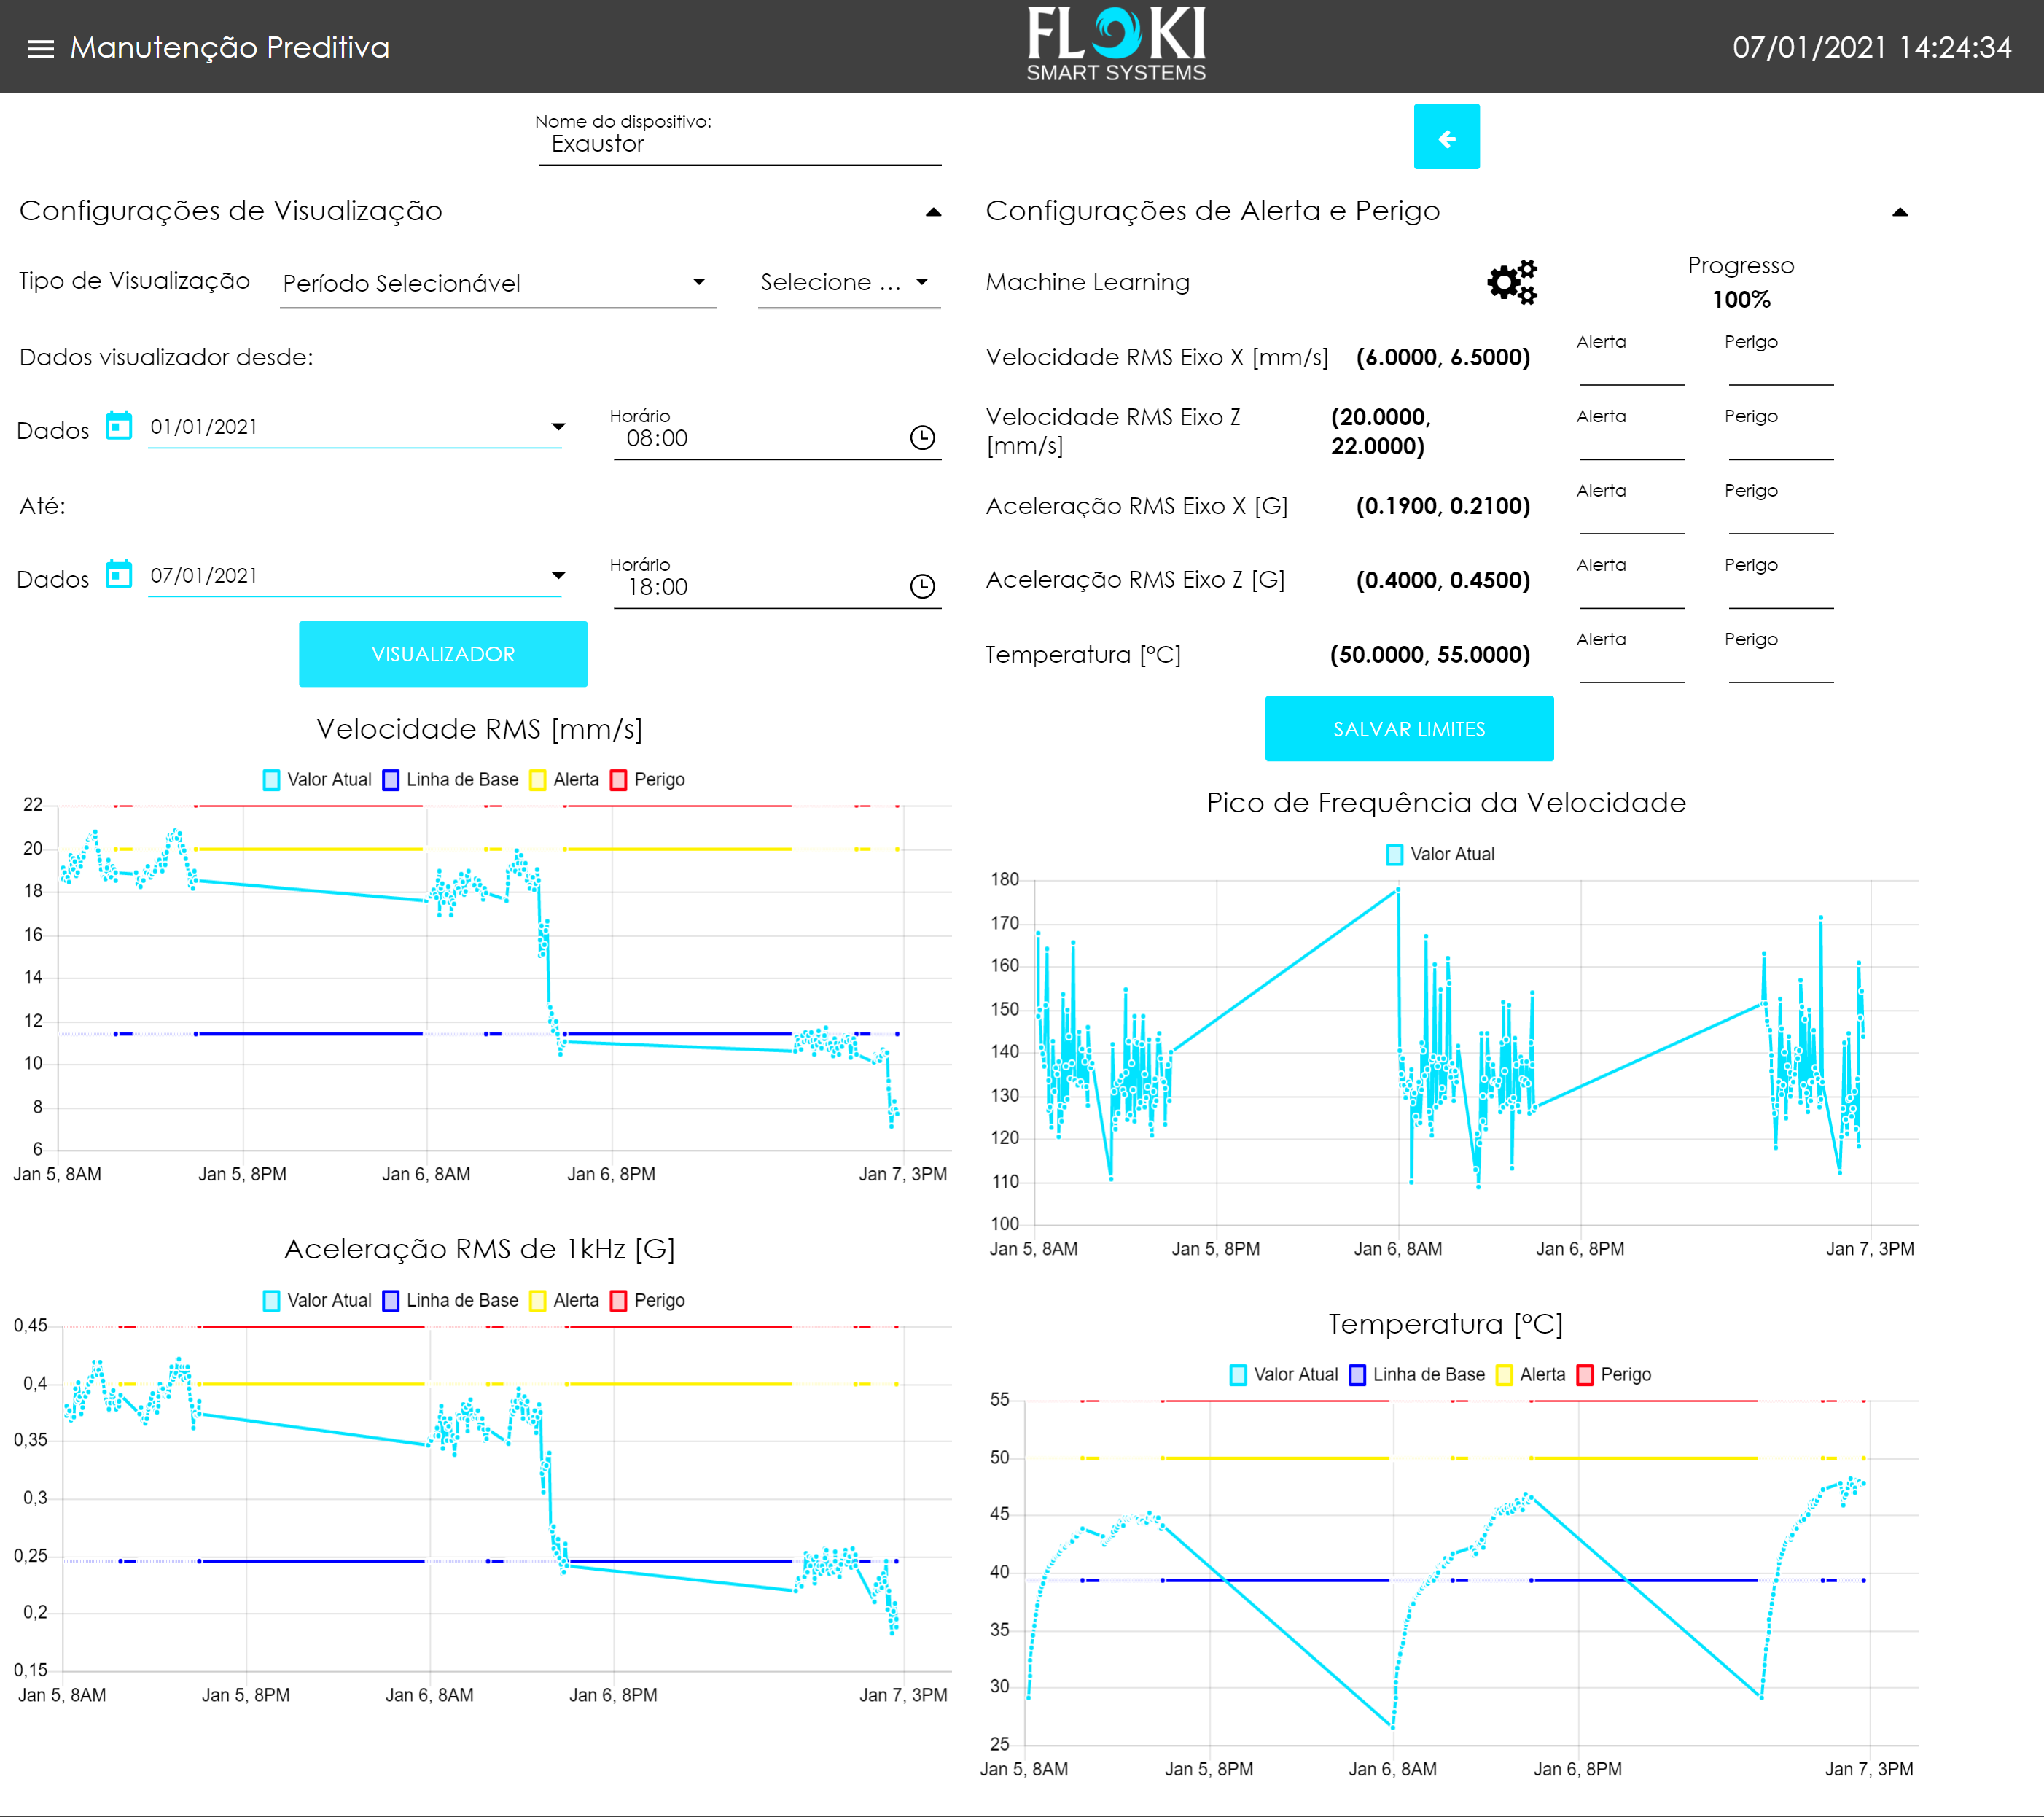
\includegraphics[scale=.15]{resultados/img/drakkar_eixo_y.png}
    \end{center}
    \fonte{Elaborado pelo Autor.} 
    \label{fig:ica}
\end{figure}

Como podemos ver, o eixo Z se encontra em estado severo de vibração, não entrando em alarme devido ao ajuste manual do operador da fábrica,
sendo agora um problema humano realizar as tarefas de forma correta.


Após a escrita de todo o trabalho, indo desde o conhecimento mínimo para o entendimento das propostas, passando pela descrição dos métodos
empregados, até os resultados preliminares, foi possível ver o funcionamento satisfatório das técnicas, mas que ainda precisam de melhorias
e a aplicação de uma CNN para classificar os resultados até agora obtidos. 

